\documentclass[notheorems, serif, table, compress]{beamer}  %dvipdfm选项是关键, 否则编译统统通不过
%%------------------------常用宏包------------------------
%%注意,  beamer 会默认使用下列宏包: amsthm,  graphicx,  hyperref,  color,  xcolor,  等等
\usepackage{fontspec, xunicode, xltxtra}  % for XeTeX
\usepackage{verbatim}
\usepackage{mathabx}
\usepackage{latexsym}
\usepackage{amsfonts, amssymb}
\usepackage{styles/iplouclistings}
\usepackage{fancybox}
\usepackage{colortbl}
\usepackage{tcolorbox}
%\usepackage[T1]{fontenc}
%\usepackage{bookman}
\usepackage{subfigure}
\usepackage{hyperref}
\usepackage{listings}
\usepackage{animate}
\usepackage[absolute, overlay]{textpos}
\usepackage{graphicx}
\usepackage{tikz}
\usepackage[americaninductors, europeanresistors]{circuitikz}
\usepackage{tikz}
\usepackage{fancybox}     %% 定义zhushadow时用到
\usepackage{pifont} %ding用到
\usepackage{mathrsfs} %一些特殊数学符号
\usepackage{extarrows}%添加上下可加文字的长等号
\usepackage{float}
\newsavebox{\mysaveboxOne}  %%为了在only中使用lstlisting
\newsavebox{\mysaveboxTwo}
\newsavebox{\mysaveboxThree}
\newsavebox{\mysaveboxFour}
\newsavebox{\mysaveboxFive}
\newsavebox{\mysaveboxSix}
\newsavebox{\mysaveboxSeven}
\newcommand\zhushadow[2][purple]{\hskip5pt\shadowbox{\color{#1}\small\kai #2\vspace{3mm}}}

%%------------------------ThemeColorFont------------------------
%% Presentation Themes
% \usetheme[<options>]{<name list>}
%\usetheme{Madrid}
\usetheme{Berkeley}
%% Inner Themes双精度计算
% \useinnertheme[<options>]{<name>}
%% Outer Themes
% \useoutertheme[<options>]{<name>}
%\useoutertheme{miniframes} 
%% Color Themes 
%\usecolortheme[<options>]{<name list>}
%% Font Themes
\usefonttheme{serif}
\setbeamertemplate{background canvas}[vertical shading][bottom=white, top=structure.fg!7] %%背景色,  上25%的蓝,  过渡到下白.
\setbeamertemplate{theorems}[numbered]
\setbeamertemplate{navigation symbols}{}   %% 去掉页面下方默认的导航条.
\usepackage{styles/zhfontcfg}
%\setsansfont[Mapping=tex-text]{文泉驿正黑}  %% 需要fontspec宏包
     %如果装了Adobe Acrobat, 可在font.conf中配置Adobe字体的路径以使用其中文字体
     %也可直接使用系统中的中文字体如SimSun, SimHei, 微软雅黑 等
     %原来beamer用的字体是sans family;注意Mapping的大小写, 不能写错
     %设置字体时也可以直接用字体名,以下三种方式等同:
     %\setromanfont[BoldFont={黑体}]{宋体}
     %\setromanfont[BoldFont={SimHei}]{SimSun}
     %\setromanfont[BoldFont={"[simhei.ttf]"}]{"[simsun.ttc]"}
%%------------------------MISC------------------------
\graphicspath{{figures/}}         %% 图片路径. 本文的图片都放在这个文件夹里了.
%%------------------------listing------------------------
%\lstset{language=[LaTeX]TeX, Python}
%%------------------------正文------------------------
\begin{document}
\XeTeXlinebreaklocale "zh"         % 表示用中文的断行
\XeTeXlinebreakskip = 0pt plus 1pt % 多一点调整的空间
%%----------------------------------------------------------
%% This is only inserted into the PDF information catalog. Can be left
%% out.
%%%
%% Delete this,  if you do not want the table of contents to pop up at
%% the beginning of each subsection:
%\AtBeginSection[]{                              % 在每个Section前都会加入的Frame
%  \frame<handout:0>{
%    \frametitle{Contents}\small
%    \tableofcontents[current, currentsubsection]
%  }
%}
%
%\AtBeginSubsection[]                            % 在每个子段落之前
%{
%  \frame<handout:0>                             % handout:0 表示只在手稿中出现
%  {
%    \frametitle{Contents}\small
%    \tableofcontents[current, currentsubsection] % 显示在目录中加亮的当前章节
%  }
%}

\setbeamertemplate{caption}{\raggedright\insertcaption\par}

%%----------------------------------------------------------
\logo{
\includegraphics[scale=0.13]{ouclogo.png}}
\title{Local Feature Extraction }
\subtitle{SIFT, SURF and LBP}
\author[]{\textcolor{olive}{常琳}}
\institute[CVBIOUC]
{
\small\textcolor{violet}{CVBIOUC\\
%Ocean University of China\\
\url{http://vision.ouc.edu.cn/~zhenghaiyong}}
}
%\date[]{}
%\titlegraphic{
%
\includegraphics[height=1.0cm]{ouc-logo.jpg}}
\frame{ \titlepage }
%%----------------------------------------------------------
%\section*{Contents}
\frame{\frametitle{Contents}\tableofcontents}
%%----------------------------------------------------------
\def\hilite<#1>{\temporal<#1>{\color{blue!15}}{\color{black}}{\color{black}}}
\newcommand{\shadow}[2][purple]{\hskip5pt\shadowbox{\color{#1}\small \kai #2\vspace{3mm}}}
\newcommand{\colorrbox}[2][purple]{\doublebox{\color{#1}\small \kai#2}}

%============================================================================

\section{Introduction} 

\begin{frame}[fragile]
\frametitle{Introduction}

\begin{figure}[!ht]
  \centering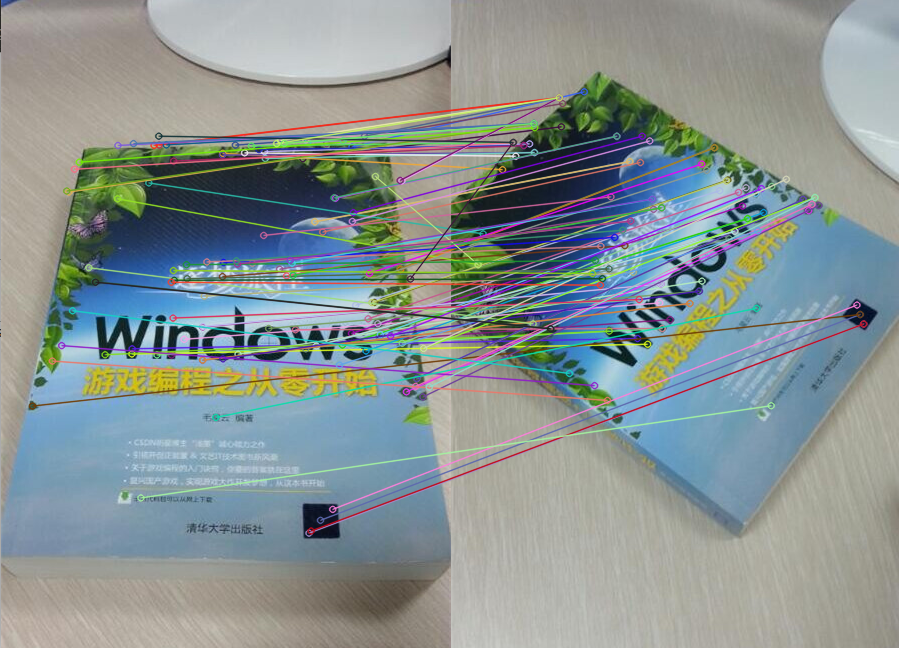
\includegraphics[width=1.5in]{surfmatch.png}
  \caption{SURF match}
 \label{surfmatch}
  \end{figure}


\begin{figure}[!ht]
  \centering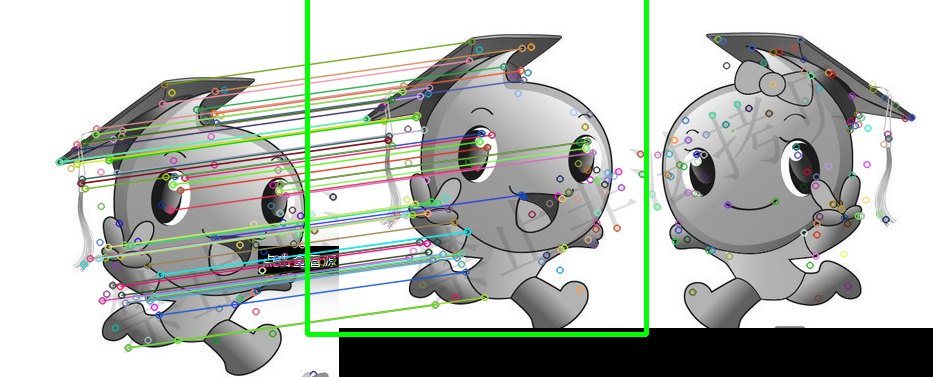
\includegraphics[width=1.8in]{siftmatch.png}
  \caption{SIFT match}
 \label{siftmatch}
  \end{figure}
\end{frame}

%=========================================================================

\section{SIFT}

\begin{frame}[fragile]
\frametitle{SIFT}

SIFT(Scale Invariant Feature Transform):

\begin{itemize}
\item An algorithm in computer vision to detect and describe local features in images. %是一种检测局部特征的算法。该算法通过求一幅图中的特征点(interest points,or corner points)及其有关scale 和 orientation 的描述子得到特征并进行图像特征点匹配。

\item Published by David Lowe in 1999.%完善于2004年

\item Accuracy, stability, scale and rotational invariance. 

\end{itemize}
\end{frame}

\begin{frame}[fragile]
\frametitle{Steps}

Steps:
\begin{enumerate}
\item Construct scale-space.

\item Detect scale-invariant interest points from scale-space extrema. %包括检测空间极值点和精确定位极值点

\item Orientation match.%关键点方向匹配

\item Compute descriptor.%关键点描述子生成

\item Match image descriptors.%描述子匹配
\end{enumerate}
\end{frame}

\subsection{Construct scale-space}
\begin{frame}[fragile]
\frametitle{Construct scale-space}
Interest points are obtained from a difference-of-Gaussians pyramid. %特征点的获取主要是从高斯差分金字塔。

%SIFT算法是在不同的尺度空间上查找关键点,尺度空间的获取需要使用高斯模糊来实现。一个图像的尺度空间$L(x,y,\sigma)$定义为一个变化尺度的高斯函数$G(x,y,\sigma)$与原图像$I(x,y)$的卷积。为了有效的在尺度空间检测到稳定的关键点,提出了高斯差分尺度空间(Different of Gaussian scale-space, DOG scale-space)。利用不同尺度的高斯差分核与图像卷积生成。

%生成金字塔的流程:
\begin{figure}[!ht]
  \centering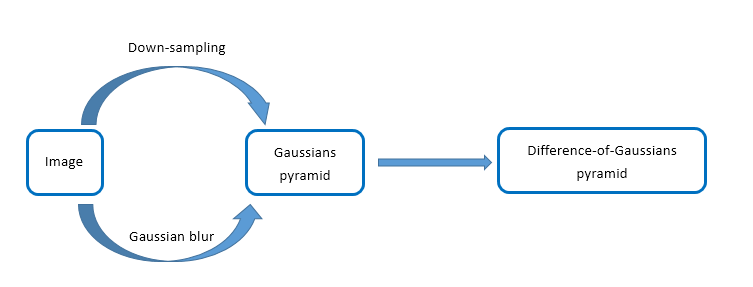
\includegraphics[width=3in]{pyramid.png}
  \caption{Construct scale-space}
 \label{step}
  \end{figure}

%在检测极值点前对原始图像的高斯平滑以致图像丢失高频信息,所以 Lowe 建议在建立尺度空间前首先对原始图像长宽扩展一倍,以保留原始图像信息,增加特征点数量。
%上图中的相关公式
Smoothed image values:%高斯模糊后的图像值
\begin{equation}
L(x,y,\sigma)=G(x,y,\sigma)*I(x,y)
\end{equation}

\end{frame}

\begin{frame}[fragile]
\frametitle{Construct scale-space}

Gaussian kernels:
\begin{equation}
G(x,y,\sigma)=\frac{1}{2\pi \sigma^{2}}e^{-\frac{(x-m/2)^{2}+(y-n/2)^{2}}{2\sigma^{2}}}
\end{equation}

%$m,n$是高斯模板大小,$(x,y)$是空间坐标,$\sigma$是尺度空间因子,其大小决定图像的模糊(平滑)程度。


The difference-of-Gaussians operator:%高斯差分算子,
\quad \\
\quad \\
$D(x,y,\sigma)=(G(x,y,k\sigma)-G(x,y,\sigma))*I(x,y)$
\begin{equation}
=L(x,y,k\sigma)-L(x,y,\sigma)
\end{equation}


%图像的金字塔模型是指将原始图像不断进行降阶采样,得到一系列大小不一的图像,由大到小,从下到上构成的塔状模型。每次降采样所得到的新图像为金字塔的一层,此时每层有一张图像,每个金字塔共 n 层,层数由图像的原始大小和塔顶图像的大小共同决定。

%为了让尺度体现其连续性(scale-invariant,也就是在任何尺度都能够有对应的特征点),高斯金字塔在简单降采样的基础上加了高斯滤波,将图像金字塔每层的一张图像使用不同参数做高斯滤波,使得金字塔的每层含有多张高斯模糊图像,将金字塔每层多张图像合称为一组(Octave 也称为子八度)。\同一个 octave 中的图片尺寸(大小)相同,但尺度(模糊程度)不同;不同的 octave 层中图片的尺寸也不同,因为后面每个 octave 层的底层图像为上一个 octave 中倒数第三张图像隔点采样的结果,即原图的 1/4(长宽分别减半)。

%在实际计算时,使用高斯金字塔每组中相邻上下两层图像相减,得到高斯差分图像。
In fact, we obtained the difference-of-Gaussians pyramid by taking subtraction between the adjacent two layers.

\end{frame}

\begin{frame}[fragile]
\frametitle{Construct scale-space}
\begin{figure}[!ht]
  \centering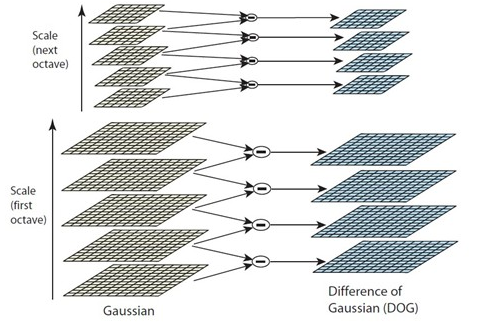
\includegraphics[width=3in]{dog.png}
  \caption{Contrust difference-of-Gaussians pyramid}
 \label{dog}
  \end{figure}


\end{frame}
%-------------------------------------------------------------------------
\subsection{Detect scale-invariant interest points from scale-space extrema}
\begin{frame}[fragile]
\frametitle{Detect scale-space extrema}%检测尺度空间极值点
 Compare the detecting point with other points in a $3*3*3$ neighbourhood. %将检测点和它同尺度的8个相邻点和上下相邻尺度对应的9×2个点共26个点比较,以确保在尺度空间和二维图像空间都检测到极值点。 一个点如果在DOG尺度空间本层以及上下两层的26个领域中是最大或最小值时,就认为该点是图像在该尺度下的一个特征

\begin{figure}[!ht]
  \centering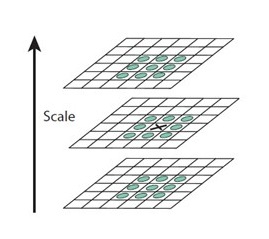
\includegraphics[width=2in]{kongjianjizhijiance.png}
  \caption{Extrema detection}
 \label{kongjianjizhijiance}
  \end{figure}


\end{frame}

\begin{frame}[fragile]
\frametitle{Detect scale-invariant interest points from scale-space extrema}%精确确定极值点
%通过拟合三维二次函数以精确确定关键点的位置和尺度(达到亚像素精度),同时去除低对比度的关键点和不稳定的边缘响应点,以增强匹配稳定性,提高抗噪声能力。

The scale coordinate of keypoints:

\begin{equation}
\sigma(o,s)=\sigma_{0}2^{o+\frac{s}{S}}  \quad o=0,1,\ldots,O-1, s=0,\ldots,S+2
\end{equation}
%σ 0 是基准层尺度,o 为 octave 的索引,s 为组内层的索引,O�S 分别为组数和组内层数
The scale of a particular layer:

\begin{equation}
\sigma_{oct}(s)=\sigma_{0}2^{\frac{s}{S}}  \quad s=0,\ldots,S+2
\end{equation}
\end{frame}

\begin{frame}[fragile]
\frametitle{Detect scale-invariant interest points from scale-space extrema}%精确确定极值点
The Taylor expansion  of D(X) is as follows:
%D(X)的泰勒展开式:
\begin{equation}
D(X)=D(X)+\frac{\partial D^{T}}{\partial X}X+\frac{1}{2}X^{T}\frac{\partial ^{2}D}{\partial X^{2}}X \quad X=(x,y,\sigma)^{T}
\end{equation}



\quad\\
%求导,令其等于0,得到极值点的偏移量为:

Deal with the derivative and let it eqaual 0. We can obtain the offset of extrema:

\begin{equation}
\^{X_1}=-\frac{\partial ^{2}D^{-1}}{\partial X_{1}^{2}}\frac{\partial D}{\partial X_1}
\end{equation}

%对应极值点处方程的值,只取前两项可得:
and

\begin{equation}
D(\^{X_1})=D+\frac{\partial D^{T}}{\partial {X_1}}\^{X_1}
\end{equation}

If $\left|D(X_1)\right|<0.3$, throw it.

%$\left|D(X)\right|$过小的点易受噪声的干扰而变得不稳定,所以将$\left|D(X)\right|$小于某个经验值的极值点删除,Lowe论文中使用0.03。 在这一过程中获得特征点的精确位置(原位置加拟合偏移量)以及尺度。

  

\end{frame}

\begin{frame}[fragile]
\frametitle{Detect scale-invariant interest points from scale-space extrema}%消除边缘响应
%一个定义不好的高斯差分算子的极值在横跨边缘的地方有较大的主曲率,而在垂直边缘的方向有较小的主曲率。DOG 算子会产生较强的边缘响应,需要剔除不稳定的边缘响应点。获取特征点处的Hessian 矩阵,主曲率通过一个 2 ∗ 2 的 Hessian 矩阵 H 求出
To suppress such points, which will be less useful for matching. We formulate the Hessian matrix:

\quad\\ 

\begin{gather*}
H=
\begin{bmatrix}
D_{xx} & D_{xy}\\
D_{xy} & D_{yy}
\end{bmatrix}
\end{gather*}

\quad \\

\begin{equation}
Tr(H)=D_{xx}+D_{yy}=\alpha +\beta 
\end{equation}

\begin{equation}
Det(H)=D_{xx}D_{yy}-(D_{xy})^{2}=\alpha \beta
\end{equation}
\end{frame}
%分别表示矩阵H对角线元素之和、矩阵H的行列式。假设$\alpha$ 是较大的特征值,$\beta$是较小的特征值,令$\alpha =r\beta$,则
\begin{frame}[fragile]
\frametitle{Detect scale-invariant interest points from scale-space extrema}%消除边缘响应
Assume that $\alpha$ is bigger than $\beta$, and $\alpha =r\beta$.

\begin{equation}
\frac{Tr(H)^{2}}{Det(H)}=\frac{(\alpha_ +\beta)^{2}}{\alpha \beta}=\frac{(r\beta +\beta)^{2}}{r\beta^{2}}=\frac{(r+1)^{2}}{r}
\end{equation}

%D的主曲率和H的特征值$\alpha ,\beta$成正比,公式$(r+1)^{2}/r$的值在两个特征值相等时最小,随着r的增大而增大。值越大,说明两个特征值的比值越大,即在某一个方向的梯度值越大,而在另一个方向的梯度值越小,而边缘恰恰就是这种情况。所以为了剔除边缘响应点,需要让该比值小于一定的阈值,因此只需检测

If
$\frac{Tr(H)^{2}}{Det(H)}>\frac{(r+1)^{2}}{r}$
, throw it.

\quad\\
(Lowe recommended $r=10$)
\end{frame}

\subsection{Orientation match}
\begin{frame}[fragile]
\frametitle{Orientation match}%关键点方向匹配

%对上面提取的每个关键点,围绕该点选择一个窗口(圆形区域,建议半径 3 ∗ 1.5σ_ oct ),窗口内各采样点的梯度方向构成一个方向直方图,根据直方图的峰值确定关键点的方向。
%L 所用的尺度为关键点所在的尺度。按尺度采样对于窗口内的每个采样点 (x, y), 其梯度向量的幅度和方向 m(x, y),θ(x, y) 公式为:

Select a window($r=3*1.5\sigma_{oct}$) around the interest point.

\begin{figure}[!ht]
  \centering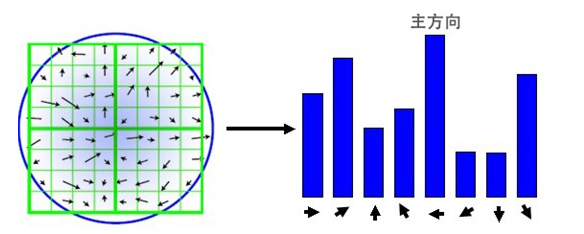
\includegraphics[width=2.5in]{guanjiandian_fangxiang_zhifangtu.png}
  \caption{Orientation histogram}
 \label{fangxiang}
  \end{figure}

With 36 bins in the histogram.
%做一个梯度方向的直方图,范围是$0-360$度,其中每10度一个柱,总共36个柱,每个采样点按照其梯度方向$\theta(x,y)$加权统计到直方图(圆形高斯加权函数,标准偏差为$\sigma=1.5\sigma\_ _{oct}$),权值为幅度$m(x,y)$和贡献因子的乘积。贡献因子是采样点到关键点(窗口中心)距离的量度(就是类似那个高斯函数的式子),距离越大,贡献因子越小。直方图的峰值代表了该关键点处邻域梯度的主方向
\end{frame}

\begin{frame}[fragile]
\frametitle{Orientation match}%关键点方向匹配

Using

\quad\\
$m(x,y)$
\begin{equation}
=\sqrt{(L(x+1,y)-L(x-1,y))^{2}+(L(x,y+1)-L(x,y-1))^{2}}
\end{equation}

\begin{equation}
\theta =\tan^{-1}((L(x,y+1)-L(x,y-1))/(L(x+1,y)-L(x-1,y)))
\end{equation}

to find the dominant orientation. 


Compute the orientation histogram based on every gradient direction $\theta(x,y)$. %Increments are weighted by the gradient magnitude $m(x,y)$ and the distance between the interest point and detection point.

Peak is the orientation. 



\end{frame}
\begin{frame}[fragile]
\frametitle{Orientation match}%关键点方向匹配

Multiple peaks are accepted if the height of secondary peaks is above 80 \% of the height of the highest peak. Express it approximately as the quadratic function curve to find actual location (the highest point).%用每个峰值和左右两个幅值拟合二次曲线,以定位峰值的实际位置(抛物线的最高点)

\end{frame}
%-------------------------------------------------------------------------
\subsection{Compute descriptor}
\begin{frame}[fragile]
\frametitle{Determine the local image region}%关键点描述子的生成
Divide the neighborhood into $4*4$ regions. Every region is a seed point.

%对梯度的求取应在特征点对应的高斯图像上进行,将关键点附近的邻域划分为 d ∗ d(d = 4) 个子区域,每个子区域作为一个种子点,每个种子点有八个方向,每个子区域的大小与关键点方向分配时相同,即每个区域有 3σ_ oct 个子像素,为每个区域分配边长为 3σ_ oct 的矩形区域进行采样(实际用边长为√ 3σ_ oct )。考虑到实际计算时,需要采用双线性插值,所需图像窗口边长为 3σ_ oct ∗ (d + 1)。
 
\begin{figure}[!ht]
  \centering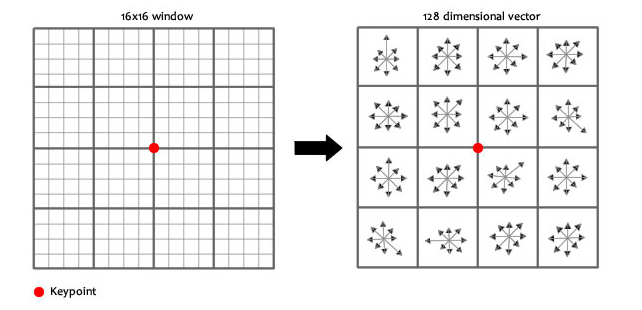
\includegraphics[width=2.5in]{128wei.png}
  \caption{Orientation histogram}
 \label{128}
  \end{figure}

\end{frame}

\begin{frame}[fragile]
\frametitle{Rotate the coordinate}%坐标轴旋转,将坐标旋转为关键点的方向,以确保旋转不变性
\begin{figure}
  \centering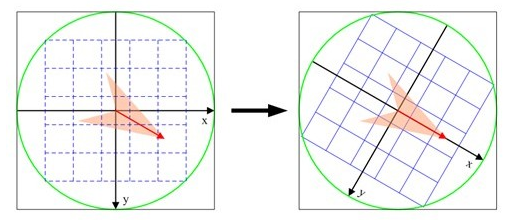
\includegraphics[width=2in]{zuobiaozhouxuanzhuan.png}
  \caption{}
 \label{zuobiaoxuanzhuan}
  \end{figure}

The new coordinate is based on the orientation of interset point.
\begin{gather*}
\begin{bmatrix}
x'\\
y'
\end{bmatrix}
=
\begin{bmatrix}
\cos\theta & -\sin\theta \\
\sin\theta & \cos\theta
\end{bmatrix}
\begin{bmatrix}
x\\
y
\end{bmatrix}
\end{gather*}

\end{frame}

\begin{frame}[fragile]
\frametitle{Allocate sampling points}%将邻域内的采样点分配到对应的子区域内,将子区域内的梯度值分配到8个方向上,计算权值。(因为旋转了,所以要重新采样再分配?)
%旋转后的采样坐标在半径为radius的圆内被分配到$d*d$的子区域,计算子区域的采样点的梯度和方向,分配到八个方向上。分配后的下标:

Rotated sampling points was allocated to $4*4$ regions.

The new coordinate is:

\begin{gather*}
\begin{bmatrix}
x''\\
y''
\end{bmatrix}
=
\frac{1}{3\sigma\_ _{oct}}
\begin{bmatrix}
x'\\
y'
\end{bmatrix}
+\frac{d}{2}
\end{gather*}
%Lowe建议子区域的像素梯度大小按$\sigma=0.5d$的高斯加权计算,即
The gradient can be computed by Gaussian weighted model as $\sigma=0.5d$:

\begin{equation}
w=m(a+x,b+y)e^{-\frac{(x')^{2}+(y')^{2}}{2x(0.5d)^{2}}}
\end{equation}

$a,b$ is the coordinate in Gaussian pyramid.
%$a,b$为关键点在高斯金字塔图像中的位置坐标。
\end{frame}

\begin{frame}[fragile]
\frametitle{Compute the gradient of 8 directions by interpolation}%插值计算每个种子点八个方向的梯度
\begin{figure}
  \centering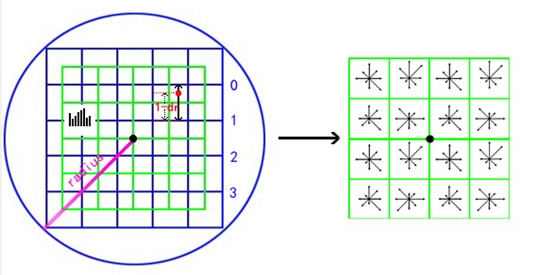
\includegraphics[width=2.5in]{miaoshuzi.png}
  \caption{}
 \label{miaoshuzi}
  \end{figure}

%将所得采样点在子区域中的下标$(x",y")$(蓝色窗口内红色点)线性插值(),计算其对每个种子点的贡献。
Linear interpolation is used on $(x'',y'')$(the red points) for computing its contribution to every seed point.  

\end{frame}

\begin{frame}[fragile]
\frametitle{Compute the gradient of 8 directions by interpolation}
\begin{figure}
  \centering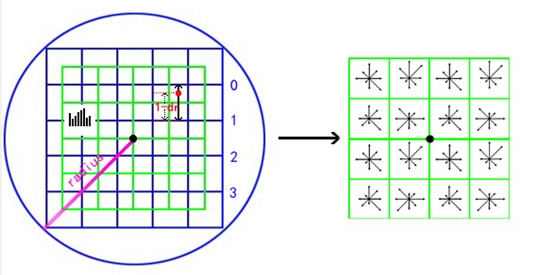
\includegraphics[width=2.5in]{miaoshuzi.png}
  \caption{}
 \label{miaoshuzi}
  \end{figure}
%如图中红色的点,落在第0行和第1行之间,对这两行都有贡献。对第0行第3列种子点的贡献因子为$dr$,对第1行第3列的贡献因子为$1-dr$,对临近两列的贡献因子为$dc$和$1-dc$对邻近两个方向贡献因子为$do$,$1-do$。最终累加在每个方向上的梯度大小为:
\begin{description}
\item[Its contributions to]
\end{description}

[0,3]: $dr$ \qquad [1,3]:  $1-dr$

Column 2: $dc$ \qquad Column 3: $1-dc$

Neighbor directions: $do$ and $1-do$. 
\end{frame}

\begin{frame}[fragile]
\frametitle{Compute the gradient of 8 directions by interpolation}
The eventual gradient magnitude added on every direction is:

\begin{equation}
weight=w*dr^{k}*(1-dr)^{1-k}*dc^{m}*(1-dc)^{1-m}*do(1-do)^{1-n}
\end{equation}
$k,m,n=0$ or $1$.
\end{frame}

\begin{frame}[fragile]
\frametitle{Normalize}%归一化
%如上统计的$4*4*8=128$个梯度信息即为该关键点的特征向量,得到的描述子向量为$H=(h_{1},h_{2},\ldots,h_{128})$。
Taken together, the local histograms computed at all the 4×4 grid points and with 8 quantized directions lead to an image descriptor$H=(h_{1},h_{2},\ldots,h_{128})$  with 4×4×8=128 dimensions for each interest point. 

Normalize $H$ to avoid the effect of illumination:
%去除光照变化的影响,需要对它们进行归一化处理,

\begin{equation}
l_{i}=\frac{h_{i}}{\sqrt{\sum_{j=1}^{128}h_{j}}}
\end{equation}
   

\end{frame}

%-------------------------------------------------------------------------
\subsection{Match image descriptors}
\begin{frame}[fragile]
\frametitle{Match image descriptors}%关键点描述子的匹配
%采用欧式距离来作为两幅图像的关键点的相似性度量。
%模板图中关键点描述子:$R_{i}=(r_{i1},r_{i2},\ldots,r_{i128})$
%实时图中关键点描述子:$S_{i}=(s_{i1},s_{i2},\ldots,s_{i128})$
%任意两描述子相似性度量:$d(R_{i},S_{i})=sqrt{\sum_{j=1}^{128}(r_{ij}-s_{ij})^{2}}$

$R_{i}=(r_{i1},r_{i2},\ldots,r_{i128})$ : Descriptors from model image.

\quad \\
$S_{i}=(s_{i1},s_{i2},\ldots,s_{i128})$ : Descriptors from another image.

\quad \\
$d(R_{i},S_{i})=\sqrt{\sum_{j=1}^{128}(r_{ij}-s_{ij})^{2}}$: Distance between $R_{i}$ and $S_{i}$.

\quad \\
If $\frac{d_{min}(R_{i},S_{i})}{d_{the\_second\_min}(R_{i},S_{j})}<Threshold$, they matched.

%实时图中距离$R_{i}$最近的点$S_{j}$/实时图中距离$R_{i}$的次最近点$S_{p}$<0.8
\end{frame}

%=========================================================================

\section{SURF}

\begin{frame}[fragile]
\frametitle{SURF}
SURF(Speeded Up Robust Features):
\begin{itemize}
\item An algorithm in computer vision to detect and describe local features in images. %是一种检测局部特征的算法。该算法通过求一幅图中的特征点(interest points,or corner points)及其有关scale 和 orientation 的描述子得到特征并进行图像特征点匹配。

\item First presrnted by Herbert Bayet al. in 2006.

\item Fast than SIFT, accuracy, stability, scale and rotational invariance. 

\end{itemize}
\end{frame}

\begin{frame}[fragile]
\frametitle{Steps}

Steps:
\begin{enumerate}
\item Construct scale-space.

\item Detect scale-invariant interest points from scale-space extrema. %包括检测空间极值点和精确定位极值点

\item Orientation match.%关键点方向匹配

\item Compute descriptor.%关键点描述子生成

\item Match image descriptors.%描述子匹配
\end{enumerate}
\end{frame}

\begin{frame}[fragile]
\frametitle{Steps}

Steps:
\begin{enumerate}
\item {\color{red}Construct scale-space.}

\item Detect scale-invariant interest points from scale-space extrema. %包括检测空间极值点和精确定位极值点

\item {\color{red}Orientation match}.%关键点方向匹配

\item {\color{red}Compute descriptor.}%关键点描述子生成

\item Match image descriptors.%描述子匹配
\end{enumerate}
\end{frame}
%------------------------------------------------------------------------------------
%\subsection{Construct scale-space}
\begin{frame}[fragile]
\frametitle{Construct scale-space}%尺度空间的建立

\begin{figure}[!ht]
  \centering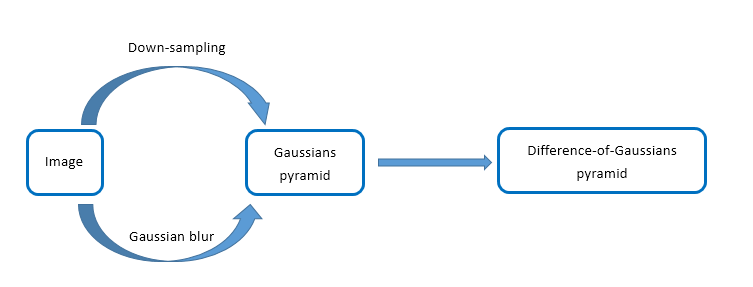
\includegraphics[width=3in]{pyramid.png}
  \caption{Construct scale-space}
 \label{step}
  \end{figure}

\end{frame}

\begin{frame}[fragile]
\frametitle{Construct scale-space}

\begin{figure}[!ht]
  \centering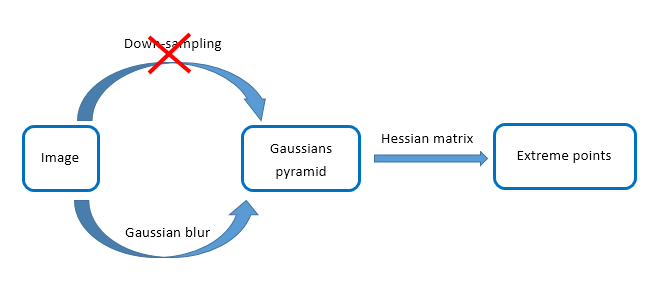
\includegraphics[width=3in]{pyramidsurf.png}
  \caption{Construct scale-space}
 \label{step}
  \end{figure}
%每一层图像上使用快速 Hessian 矩阵来检测图像的极值点。
%SURF中,图片的大小是一直不变的,不同Octave层的带检测图片是改变高斯模糊尺度大小得到的。算法允许尺度空间多层图像同时被处理,不需要对图像进行二次抽样。没有经过降采样
The discriminant of Hessian matrix to detect extrema can be approximated as follows:

\begin{equation}
Det(Happrox)=D_{xx}D_{yy}-(0.9D_{xy})^{2}
\end{equation}

$D_{xx},D_{xy},D_{yy}$ are the convolution results of Gaussian kernels and original image.
\end{frame}

%------------------------------------------------------------------------
\begin{frame}[fragile]
\frametitle{Orientation match}%选取特征点的主方向,为了保持旋转不变性
%sift选取特征点的主方向是采用在特征点领域内统计其梯度直方图,取直方图bin值最大的以及超过最大值80%的哪些方向作为主方向。
%在surf中,是统计特征点领域内的harr小波特征。即在特征点的领域(比如半径为6s的圆内,s为该点所在的尺度)内,统计60度扇形内所有点的水平haar小波特征和垂直小波特征总和,haar小波的尺寸边长为4s,这样扇形得到了一个值。然后60度扇形以一定间隔进行旋转(5度),最后将最大值那个扇形的方向作为该特征点的主方向。

\begin{figure}[!ht]
  \centering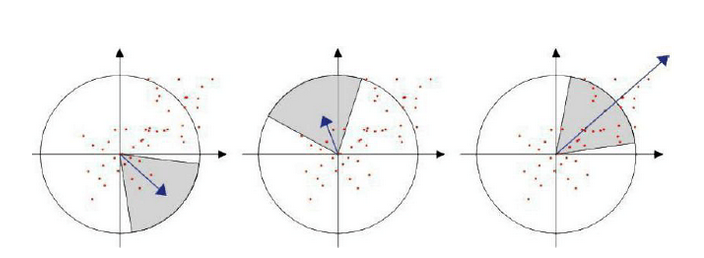
\includegraphics[width=2.5in]{haar.png}
  \caption{Estimate the dominant orientation}
 \label{step}
  \end{figure}

Angle: $\frac{\pi}{3}$.

Radius: 6s (s is the scale at which the interest pointwas detected). 

Calculate the Haar-wavelet responses in x and y direction. The maximum sum of all responses is the dominant orientation.
\end{frame}

\begin{frame}[fragile]
\frametitle{Compute descriptor}%构造特征点描述算子

%在sift中,是在特征点周围选取16*16的邻域,并把该邻域化为4×4个的小区域,每个小区域统计8个方向梯度,最后得到128维的向量作为描述子。
%在surf中,是在特征点周围取一个正方形框,边长20s,方向为该特征点的主方向,然后把框分为16个子区域,每个子区域统计25个像素的水平方向和垂直方向的haar小波特征,这里的水平和垂直方向都是相对主方向而言的。该haar小波特征为水平方向值之和,水平方向绝对值之和,垂直方向之和,垂直方向绝对值之和。这样每个小区域就有4个值,所以每个特征点就是16*4=64维的向量。比sift少了一半,会大大加快匹配速度。

Construct a square region (20s) aligned to the selected orientation. $4*4$ square sub-regions, $5*5$ regularly spaced sample points.


\begin{figure}[!ht]
  \centering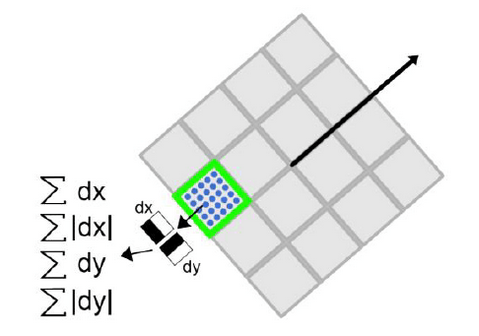
\includegraphics[width=1.8in]{descriptorsurf.png}
  \caption{Compute descriptor}
 \label{step}
  \end{figure}

We call $dx$ the Haar wavelet response in horizontal direction and $dy$ the Haar wavelet response in vertical direction.

Vector $\textbf{v}=(\sum dx, \sum \left|dx\right|, \sum dy, \sum \left|dy\right|)$
\end{frame}

%=========================================================================
\section{LBP}
\begin{frame}[fragile]
\frametitle{LBP}

LBP(Local Binary Pattern):

\begin{itemize}
\item One of the method about local information extraction. It reflects the gray value relationship between the pixel and points around it.%LBP就是一种局部信息,它反应的内容是每个像素与周围像素的关系。

\item Proposed by Ojala et al.

\item LBP operator has significant effect in the description of texture feature extraction.%在描述纹理特征提取方面有显著效果。
\end{itemize}
\end{frame}
\subsection{Encoding formula}
\begin{frame}[fragile]
\frametitle{Encoding formula}
%对任意的LBP算子,它的编码公式为:
The encoding formula for any LBP operator is: 
\begin{equation}
LBP_{P,R}=\sum_{i=0}^{p-1}s(g_{i}-g_{c})2^{i}, s(x)= \left\{ \begin{array}{ll}
1 & \textrm{$x\geq0$}\\
0 & \textrm{$x<0$}\\
\end{array} \right.
\end{equation}
$P$: The number of pixels in the $(P,R)$ neighborhood.
 
$R$: The neighborhood radius.

$g_{i}$$(i=1,2 \ldots P-1)$: The pixel values in the neighborhood with a threhold $g_{c}$.
%P表示邻域内包含的像素个数,R表示邻域半径.式中gi表示P个以中心像素gc为圆心,R为半径的圆周上的像素值
\end{frame}

\subsection{Calculation process}
\begin{frame}[fragile]
\frametitle{Calculation process}
%具体计算过程如图3,P8,R=1,将图3左边模板阈值化,即使各邻域像素点与中心像素做比较得到s的值,大于0s=1,小于0则s=0,得到图3中间图,确定各像素点的权重,如图3右图,计算阈值化后各像素与对应权重的点积,(将图3中间图的二进制数转化为十进制),即为LBP算子,可以用这个值来反应该区域的纹理信息.将LBP特征进行直方图统计,即统计LBP特征0~255各占的比例,就可以得到一个具有256维特征的数据.


\begin{figure}[!ht]
  \centering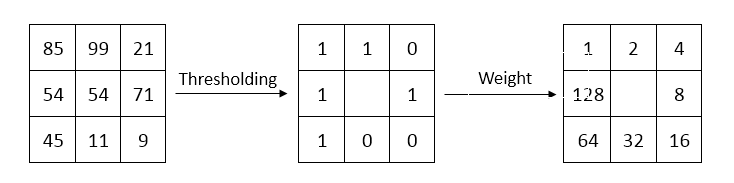
\includegraphics[width=3in]{lbp.png}
  \caption{Basic LBP operator ($P=8$ and $R=1$)}
 \label{3}
  \end{figure}

The LBP operator$=1+2+8+64+128=203$

Count the ratio of LBP opetator between 0 and 255 to a histogram.

Obtain a data with 256-dimensional features.
\end{frame}



\begin{frame}[fragile]
\frametitle{Calculation process}

Convert all the images size into $64*64$ and each image is divided into $8*8$ local regions.
%先将藻种图片大小统一一处理成64*64,再将图片划分成8*8块区域,对每个小区域进行LBP处理,再将每个小区域的直方图进行串联,得到整个图像的LBP直方图
\begin{figure}[!ht]
\centering
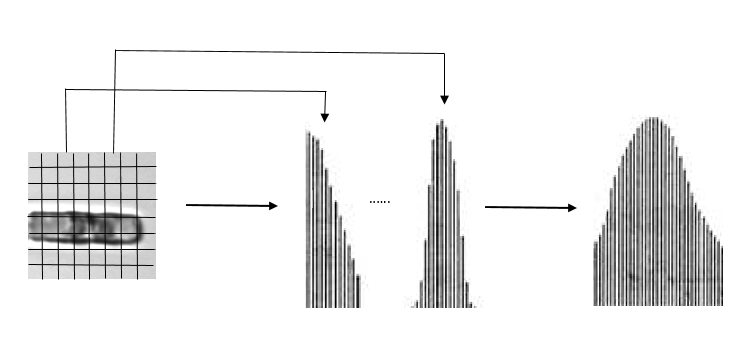
\includegraphics[width=3.5in]{lbpglobal.png}
\caption{Global image description based on LBP}
\label{fig_5}
\end{figure}

Concatenate the regional histograms to build a global histogram.

%提取特征后得到特征矩阵,可以用来进行图像识别,分类等问题的研究。

\end{frame}




%=========================================================================
\end{document}
